\title{Syntax and Semantics Exam}
\author{
        Benjamin Bennetzen \\
        Student ID: 20204861 \\
        Computer Science, 4th semester\\
}
\date{\today}

\documentclass[12pt]{article}

\usepackage{tikz}
\usepackage{listings}
\usepackage{mathpartir}
\usepackage{ebproof}
\usepackage{amsmath}
\usepackage[utf8]{inputenc}
\usepackage{amssymb}
\usepackage{graphicx}
\usepackage{stmaryrd}

\newcommand{\R}{\mathbb{R}}
\newcommand{\F}{\mathbb{F}}
\newcommand{\num}[1]{\mathcal{N}\llbracket #1 \rrbracket}
\newcommand{\ul}[1]{\underline{#1}}

\begin{document}
\maketitle

\section{Exercise}
\subsection{}

\begin{center}
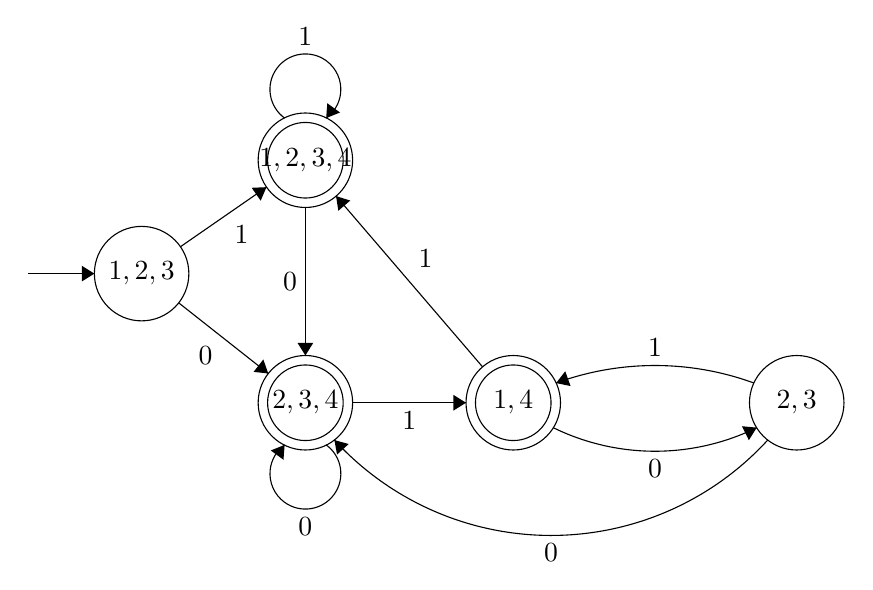
\begin{tikzpicture}[scale=0.2]
\tikzstyle{every node}+=[inner sep=0pt]
\draw [black] (26.1,-20.6) circle (3);
\draw (26.1,-20.6) node {$1,2,3$};
\draw [black] (36.5,-13.4) circle (3);
\draw (36.5,-13.4) node {$1,2,3,4$};
\draw [black] (36.5,-13.4) circle (2.4);
\draw [black] (36.5,-28.8) circle (3);
\draw (36.5,-28.8) node {$2,3,4$};
\draw [black] (36.5,-28.8) circle (2.4);
\draw [black] (49.7,-28.8) circle (3);
\draw (49.7,-28.8) node {$1,4$};
\draw [black] (49.7,-28.8) circle (2.4);
\draw [black] (67.7,-28.8) circle (3);
\draw (67.7,-28.8) node {$2,3$};
\draw [black] (18.9,-20.6) -- (23.1,-20.6);
\fill [black] (23.1,-20.6) -- (22.3,-20.1) -- (22.3,-21.1);
\draw [black] (28.57,-18.89) -- (34.03,-15.11);
\fill [black] (34.03,-15.11) -- (33.09,-15.15) -- (33.66,-15.97);
\draw (32.44,-17.5) node [below] {$1$};
\draw [black] (28.46,-22.46) -- (34.14,-26.94);
\fill [black] (34.14,-26.94) -- (33.83,-26.05) -- (33.21,-26.84);
\draw (30.16,-25.2) node [below] {$0$};
\draw [black] (35.177,-10.72) arc (234:-54:2.25);
\draw (36.5,-6.15) node [above] {$1$};
\fill [black] (37.82,-10.72) -- (38.7,-10.37) -- (37.89,-9.78);
\draw [black] (36.5,-16.4) -- (36.5,-25.8);
\fill [black] (36.5,-25.8) -- (37,-25) -- (36,-25);
\draw (36,-21.1) node [left] {$0$};
\draw [black] (39.5,-28.8) -- (46.7,-28.8);
\fill [black] (46.7,-28.8) -- (45.9,-28.3) -- (45.9,-29.3);
\draw (43.1,-29.3) node [below] {$1$};
\draw [black] (37.823,-31.48) arc (54:-234:2.25);
\draw (36.5,-36.05) node [below] {$0$};
\fill [black] (35.18,-31.48) -- (34.3,-31.83) -- (35.11,-32.42);
\draw [black] (47.75,-26.52) -- (38.45,-15.68);
\fill [black] (38.45,-15.68) -- (38.59,-16.61) -- (39.35,-15.96);
\draw (43.65,-19.66) node [right] {$1$};
\draw [black] (65.158,-30.384) arc (-63.92761:-116.07239:14.694);
\fill [black] (65.16,-30.38) -- (64.22,-30.29) -- (64.66,-31.18);
\draw (58.7,-32.38) node [below] {$0$};
\draw [black] (52.421,-27.545) arc (110.05999:69.94001:18.305);
\fill [black] (52.42,-27.55) -- (53.34,-27.74) -- (53,-26.8);
\draw (58.7,-25.93) node [above] {$1$};
\draw [black] (65.861,-31.166) arc (-42.4609:-137.5391:18.653);
\fill [black] (38.34,-31.17) -- (38.51,-32.09) -- (39.25,-31.42);
\draw (52.1,-37.73) node [below] {$0$};
\end{tikzpicture}
\end{center}

\section{Exercise}
\begin{center}
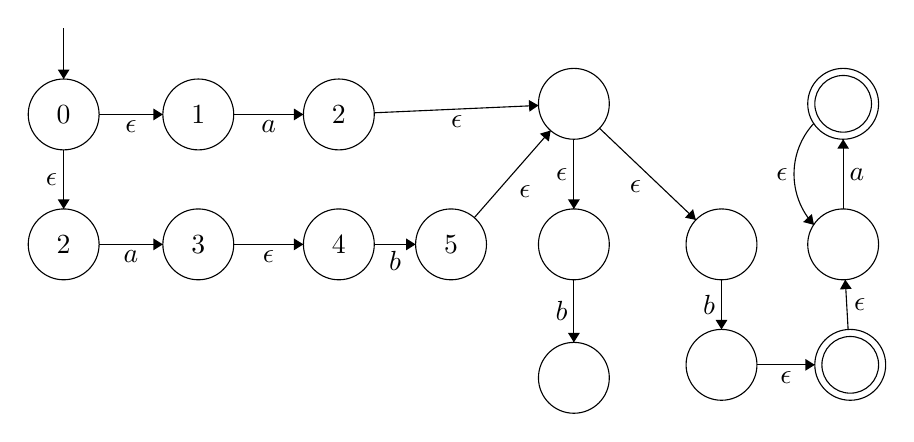
\begin{tikzpicture}[scale=0.15]
\tikzstyle{every node}+=[inner sep=0pt]
\draw [black] (16,-11.2) circle (3);
\draw (16,-11.2) node {$1$};
\draw [black] (27.9,-11.2) circle (3);
\draw (27.9,-11.2) node {$2$};
\draw [black] (4.6,-22.2) circle (3);
\draw (4.6,-22.2) node {$2$};
\draw [black] (16,-22.2) circle (3);
\draw (16,-22.2) node {$3$};
\draw [black] (27.9,-22.2) circle (3);
\draw (27.9,-22.2) node {$4$};
\draw [black] (37.4,-22.2) circle (3);
\draw (37.4,-22.2) node {$5$};
\draw [black] (4.6,-11.2) circle (3);
\draw (4.6,-11.2) node {$0$};
\draw [black] (70.6,-22.2) circle (3);
\draw [black] (70.6,-10.3) circle (3);
\draw [black] (70.6,-10.3) circle (2.4);
\draw [black] (71.2,-32.4) circle (3);
\draw [black] (71.2,-32.4) circle (2.4);
\draw [black] (60.3,-22.2) circle (3);
\draw [black] (60.3,-32.4) circle (3);
\draw [black] (47.8,-22.2) circle (3);
\draw [black] (47.8,-33.5) circle (3);
\draw [black] (47.8,-10.3) circle (3);
\draw [black] (19,-11.2) -- (24.9,-11.2);
\fill [black] (24.9,-11.2) -- (24.1,-10.7) -- (24.1,-11.7);
\draw (21.95,-11.7) node [below] {$a$};
\draw [black] (7.6,-22.2) -- (13,-22.2);
\fill [black] (13,-22.2) -- (12.2,-21.7) -- (12.2,-22.7);
\draw (10.3,-22.7) node [below] {$a$};
\draw [black] (30.9,-22.2) -- (34.4,-22.2);
\fill [black] (34.4,-22.2) -- (33.6,-21.7) -- (33.6,-22.7);
\draw (32.65,-22.7) node [below] {$b$};
\draw [black] (19,-22.2) -- (24.9,-22.2);
\fill [black] (24.9,-22.2) -- (24.1,-21.7) -- (24.1,-22.7);
\draw (21.95,-22.7) node [below] {$\epsilon$};
\draw [black] (4.6,-3.9) -- (4.6,-8.2);
\fill [black] (4.6,-8.2) -- (5.1,-7.4) -- (4.1,-7.4);
\draw [black] (7.6,-11.2) -- (13,-11.2);
\fill [black] (13,-11.2) -- (12.2,-10.7) -- (12.2,-11.7);
\draw (10.3,-11.7) node [below] {$\epsilon$};
\draw [black] (4.6,-14.2) -- (4.6,-19.2);
\fill [black] (4.6,-19.2) -- (5.1,-18.4) -- (4.1,-18.4);
\draw (4.1,-16.7) node [left] {$\epsilon$};
\draw [black] (70.6,-19.2) -- (70.6,-13.3);
\fill [black] (70.6,-13.3) -- (70.1,-14.1) -- (71.1,-14.1);
\draw (71.1,-16.25) node [right] {$a$};
\draw [black] (71.02,-29.41) -- (70.78,-25.19);
\fill [black] (70.78,-25.19) -- (70.32,-26.02) -- (71.32,-25.96);
\draw (71.49,-27.27) node [right] {$\epsilon$};
\draw [black] (68.125,-20.554) arc (-137.19791:-222.80209:6.334);
\fill [black] (68.13,-20.55) -- (67.95,-19.63) -- (67.21,-20.31);
\draw (65.94,-16.25) node [left] {$\epsilon$};
\draw [black] (60.3,-25.2) -- (60.3,-29.4);
\fill [black] (60.3,-29.4) -- (60.8,-28.6) -- (59.8,-28.6);
\draw (59.8,-27.3) node [left] {$b$};
\draw [black] (47.8,-25.2) -- (47.8,-30.5);
\fill [black] (47.8,-30.5) -- (48.3,-29.7) -- (47.3,-29.7);
\draw (47.3,-27.85) node [left] {$b$};
\draw [black] (63.3,-32.4) -- (68.2,-32.4);
\fill [black] (68.2,-32.4) -- (67.4,-31.9) -- (67.4,-32.9);
\draw (65.75,-32.9) node [below] {$\epsilon$};
\draw [black] (49.97,-12.37) -- (58.13,-20.13);
\fill [black] (58.13,-20.13) -- (57.89,-19.22) -- (57.2,-19.94);
\draw (53.01,-16.73) node [below] {$\epsilon$};
\draw [black] (47.8,-13.3) -- (47.8,-19.2);
\fill [black] (47.8,-19.2) -- (48.3,-18.4) -- (47.3,-18.4);
\draw (47.3,-16.25) node [left] {$\epsilon$};
\draw [black] (39.37,-19.94) -- (45.83,-12.56);
\fill [black] (45.83,-12.56) -- (44.92,-12.83) -- (45.68,-13.49);
\draw (43.14,-17.7) node [right] {$\epsilon$};
\draw [black] (30.9,-11.06) -- (44.8,-10.44);
\fill [black] (44.8,-10.44) -- (43.98,-9.97) -- (44.03,-10.97);
\draw (37.89,-11.29) node [below] {$\epsilon$};
\end{tikzpicture}
\end{center}


\end{document}
